% !TEX encoding = UTF-8 Unicode
\documentclass[a4paper]{article}

\usepackage[utf8]{inputenc}
\usepackage{erk}
\usepackage{times}
\usepackage{graphicx}
\usepackage{cite}
\usepackage{array}
\usepackage[top=22.5mm, bottom=22.5mm, left=22.5mm, right=22.5mm]{geometry}

\usepackage[english]{babel}

% local definitions
\def\footnotemark{}%  to avoid footnote on cover page

\begin{document}
%make title
\title{An evaluation of feature types for mood estimation on a newly presented dataset of emotion and color responses to music}

\author{Primož Godec$^{1}$, Matevž Pesek$^{1}$, Mojca Poredoš$^{1}$, Gregor Strle$^{2}$,\\ Jože Guna$^{3}$, Emilija Stojmenova$^{3}$, Matevž Pogačnik$^{3}$ and Matija Marolt$^{1}$} % use ^1, ^2 for author(s) from different institutions

\affiliation{$^{1}$University of Ljubljana, Faculty of computer and information science \\ 
$^{2}$Institute of Ethnomusicology, Scientfic Research Centre of the Slovenian Academy of Sciences and Arts \\
$^{3}$University of Ljubljana, Faculty of Electrotechnics}

\email{E-mail: \{matevz.pesek, matija.marolt\}@fri.uni-lj.si, \{primoz.godec, mojca.poredos\}@lgm.fri.uni-lj.si \\ gregor.strle@zrc-sazu.si,  \{joze.guna, emilija.stojmenova, matevz.pogacnik\}@fe.uni-lj.si}

\maketitle

\begin{abstract}{Abstract}
This paper presents a new dataset gathered containing perceived and induced emotions for 200 audio clips. The gathered dataset also provides users' association of color for each clip, along with users' demographic and personal data, such as users' emotion state, preferred genres, music experience and daily inference, and others. With an online survey we collected more than 7000 responses for a dataset of 200 audio excerpts, thus providing about 37 user responses per clip. We introduced a new methodology for gathering user perception of emotions in a form of two new interfaces - the MoodGraph and MoodStripe. We present a preliminary evaluation of classifying the present emotions with a regression algorithm using MFCC and Chroma on the gathered dataset, and perform a comparison towards other datasets and algorithms. 
\end{abstract}

\section{Introduction}

This paper tackles the problem of mood estimation in the field of music information retrieval (MIR). There are several applications of the mood estimation, for example in order to boost the efficiency of music recommendation systems. In order to develop such music recommendation system, an annotated dataset is needed for training. Several datasets were previously gathered, yet, to our knowledge, no dataset contained demographic and background data of the users who provided the annotations. Since the mood itself is highly subjective, we believe a dataset annotated by a large group of people can provide a solid base for further research in this field.

In order to obtain a statistically significant amount of user responses per song, we performed user response gathering over a dataset for 200 audio clips. In addition to responses on music clips, we collected some other participants' demographic data and perception of mood. This data might help us to understand difference in responses to audio clips and possibly find correlations between users with similar background. In order to evaluate the usefulness of the collected data and possibly highlight the importance of the relations between the modalities and the user's personal data, we performed a preliminary evaluation of the mood estimation algorithm using the regression for valence-arousal prediction, as described in \cite{schmidt2009projection}. This algorithm was tested on our dataset and Mood Swing Turk dataset \cite{schmidt2011modeling}.

Several datasets for mood estimation were previously presented. We intend to overcome some drawbacks of these datasets, such as a small amount of annotators, lack of background information (e.g. genre preference might bias one annotators perception regarding the perceived emotions). Eerola et al \cite{eerola2010comparison} performed a gathering of the film music dataset. Each sound track provides a single mean rating with label and values in three-dimensional valence-arousal-tension model. The dataset contains values for 361 film music clips. The Mood Swings Turk Dataset contains on average 17 valence-arousal ratings for each of the 240 audio clips \cite{schmidt2011modeling}. Clips in this dataset are mostly excerpts from popular music. The Cal500 provides mood labels for 500 western popular songs \cite{turnbull2008semantic} encompassing 3 annotations per song. The MTV Music Dataset contains 5 bipolar valence-arousal ratings for 192 popular songs \cite{schuller2010mister}. These songs were obtained from the MTV channel playlists.


Mood estimation and perception has been explored on some of the mentioned datasets. However, there are several undiscovered relations that brought the problem to our attention. Music mood estimation has become a recognised task in the past year; the music information retrieval evaluation exchange (MIREX) organises mood classification task since 2007. Several machine-learning-driven approaches have already been presented for the mood estimation task. Schmi\-dt et al. \cite{schmidt2009projection} use regression for mood classification. Panda et al. \cite{panda2013multi} use support vector machines, k-nearest neighbours, C4.5 and naive bayes. Support vector machine was also used by \cite{laurier2007audio}. Barthet et al. \cite{barthet2013design} use support vector regression for classification. 

The paper is structured as follows: section 2 describes the survey and it design, section 3 provides analyses of the gathered data and survey evaluation and section 4 concludes the paper and describes our future work.


\section{Online survey}

For the user responses gathering procedure, an online survey was used. In order to fully anticipate possible drawbacks of previously collected annotations, we carefully picked the set of labels for emotions by performing a preliminary study over a large label set and identifying the key labels most fitting the majority of participants.

Some basic emotion labels exist, e.g. \cite{dalgleish1999handbook}; however, there is no standard set in music and mood research to our knowledge. Others choose label sets intuitively, without any explanations \cite{wu2013spectral}. In order to use an optimal set of labels, we prepared preliminary survey.

Participants were asked describe their emotional state on scale from 1 to 7 for each of 48 emotional labels. We also observed responses about color perception on a continuous color wheel used to describe connection between mood and colors. Depending on results of this questionnaire we selected 17 basic emotion labels which strongly correlate to three basic components that explain 64\% of the variance to the dataset. Depending on participants' responses and results we also decided to restrict continuous color wheel; we developed a discrete-scale color wheel containing 49 colors. 

\subsection{The survey}

By incorporating the conclusions of the preliminary survey, we performed a second  online survey on a larger set of participants. We structured the survey into three sections. We captured participants' personal background and demographic information in first part. Users were asked to answer the demographic questions about the following aspects: age, area of living and native language along with information about users' music education, genre preference, and the amount of time listening to the music. We speculate about the importance of such data being gathered along with the mood perception responses for the annotated dataset. 

Second part contains questions about participants' perception of mood and connection between color and mood. First, the participants were asked about their current mood state in a set of three separate tasks. A participant was asked to pin-point a location best matching his current mood in the valence-arousal space. The valence-arousal space is a 2D plane, describing the pleasantness on one and activeness on the second axis. We also inquired about the user's perception of current mood by selecting best-matching color in a color wheel. 

Instead of gathering the participants' mood using the standardised Likert scale questionnaire, we introduced a new interface, described in \cite{pesek2014gathering}, named the MoodStripe (see Fig. \ref{moodstripe}). The participant was asked to drag each label describing one emotion onto a one-dimensional canvas. The canvas possesses a continuous scale between \textit{completely absent} and \textit{significantly expressed}.

The second part contained also two tasks of capturing their perception of emotions. First, the user was asked to place 10 basic emotional labels onto valence-arousal space according to their view of the activeness and pleasantness of the emotion. For this task we developed a second interface named \textit{the  MoodGraph} (see Fig. \ref{moodgraph}), extending the moodStripe into a two dimensional canvas. The user was also asked to pick a best-matching color for each music excerpt.

\begin{figure}[ht]
\centering
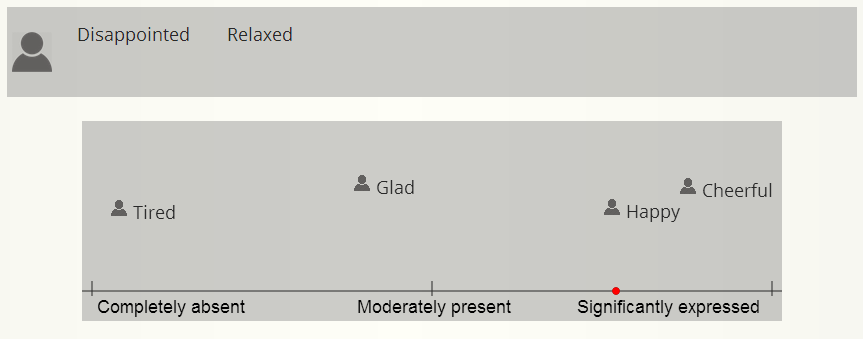
\includegraphics[width=80mm]{moodstripe.png}
\caption{The new interface used in our survey, named \textit{the MoodStripe}. With the drag-and-drop technique, a user can place emotion labels onto the plane depending on how the dragged emotion expressed. Placing the label towards the left side of the canvas reflects the absence of the emotions, where as placing it towards the right expresses the presence.}
\label{moodstripe}
\end{figure}

\begin{figure}[ht]
\centering
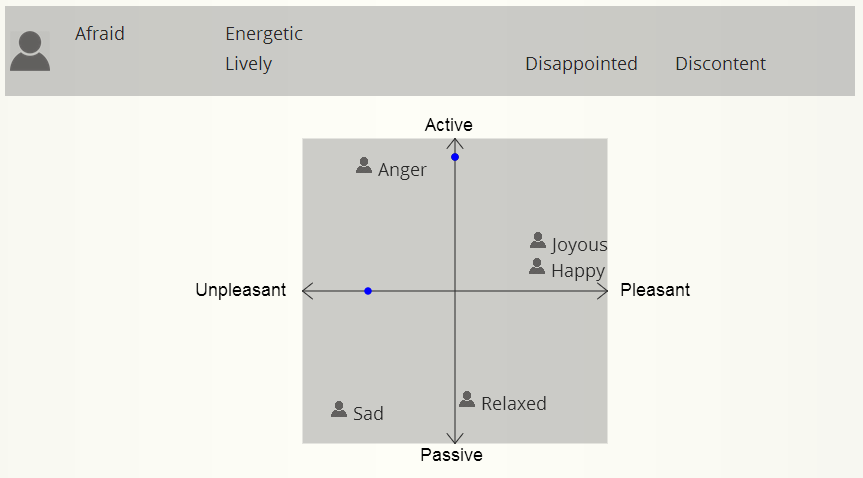
\includegraphics[width=80mm]{moodgraph.png}
\caption{The MoodGraph - a two-dimensional extension of the moodStripe interface, with one category of nominal values. On the x axis \textit{valence} (pleasantness) raises from the left to the right, on the y axis raises \textit{arousal} (activeness) from the bottom to the top.}
\label{moodgraph}
\end{figure}

In the third part of our survey, the participant was asked to respond to audio clips. The clips are 15 second long and was randomly selected from the dataset of 200 clips. To avoid overwhelming the participant, only 10 clips are presented during each participation. All selected audio clips are unknown for most of the participants, to avoid bias due to the familiarity of song. We gathered music from four sources. Eighty songs were chosen from the free online music service Jamendo. We selected songs from as many genre as possible. Next 80 clips was from film music dataset and is described here \cite{eerola2010comparison}. We also provide 20 clips from collection of slovenian folk music collection and 20 of the contemporary electro-acoustic music collection. 

The participant performed two tasks on each provided audio clip: selecting the best-matching color reflecting the audio, and to describe the perceived and induced emotions of the audio. The latter was performed by using a two-category moodgraph. We provided two categories of labels, one with perceived and the other with induced emotion labels. The user was asked to select at least one label from each category and place them into the valence-arousal space (Fig. \ref{moodgraph}). 

\section{Results}

\begin{table*}[t]
\caption{Results for our and Mood Swing dataset in prediction of valence-arousal with regression using MFCC and Chroma. Three rates were used to measure accuracy: average distance to mean valence-arousal value, average distance to nearest valence-arousal value, average distance to mean valence-arousal value measured in number of standard deviations.}

\begin{tabular}{| l | c | c | c | c | c | c |}
\hline
Feature & \multicolumn{3}{c |}{Our dataset} & \multicolumn{3}{c |}{Mood Swing dataset} \\
\hline
 & Avg. distance & Near. distance & Avg. dist in sdt & Avg. distance & Near. distance & Avg. dist in sdt \\
\hline
MFCC & 0.2243 & 0.0611 & 0.5357 & 0.2448 & 0.0641 & 0.6514\\
Chroma & 0.2215 & 0.0614 & 0.4993 & 0.3316 & 0.1026 & 0.8940\\
\hline
\end{tabular}
\label{regressionresults}
\end{table*}

We collected 7187 responses from 1357 participants in our survey. The dataset contains 200 audio clips, resulting in collecting 37 responses per audio clip on average. To our knowledge, there is no mood-music dataset with such high ratio per clip. Each response contains at least two positioned labels - one describing a perceived and one an induced emotion, and a picked color tone for the audio clip. 

The following section presents a preliminary demographic analysis, along with a performed experiment using the regression for mood estimation on the collected dataset.

\subsection{Demographic analysis}

The basic demographic characteristics of the 952 participants are as follows. The average age of participants was 26.5 years, the youngest had 15, the oldest 64 years. 65\% of participants are women, 66\% are from urban areas. 50\% have no music education, 47\% do not play instruments or sing. The amount of music listening per day is evenly spread from less than 1 hour to over 4 hours. 3\%
claimed they were under the influence of drugs when taking the survey.

\subsection{Predicting valence-arousal values using regression}

We performed a simple mood estimation using the regression on the collected dataset. We implemented the regression algorithm described by \cite{schmidt2009projection}. The least squares method on mel-frequency cepstral coefficients (MFCC) \cite{logan2000mel} and Chroma \cite{bello2005robust} features were used. The MFCCs was calculated with the cepstral coefficients 20, Chroma was calculated using 12 bins. Features was calculated using LibROSA python library on a 15 seconds audio clips from dataset. The dataset was divided into 2 training (70\%) and  testing (30\%) sets for the least squares method \cite{abdi2007method}. Training performed by using the mean values of valence and arousal components of the responses. The algorithm separately evaluated the valence and arousal components using following equation:

\begin{equation} 
y = X b
\end{equation} 

where $X$ is features matrix. Each row in $X$ presents feature vector for single audio clip. $b$  is the transformation vector from feature matrix to prediction vector $y$.

\begin{figure}[ht]
\centering
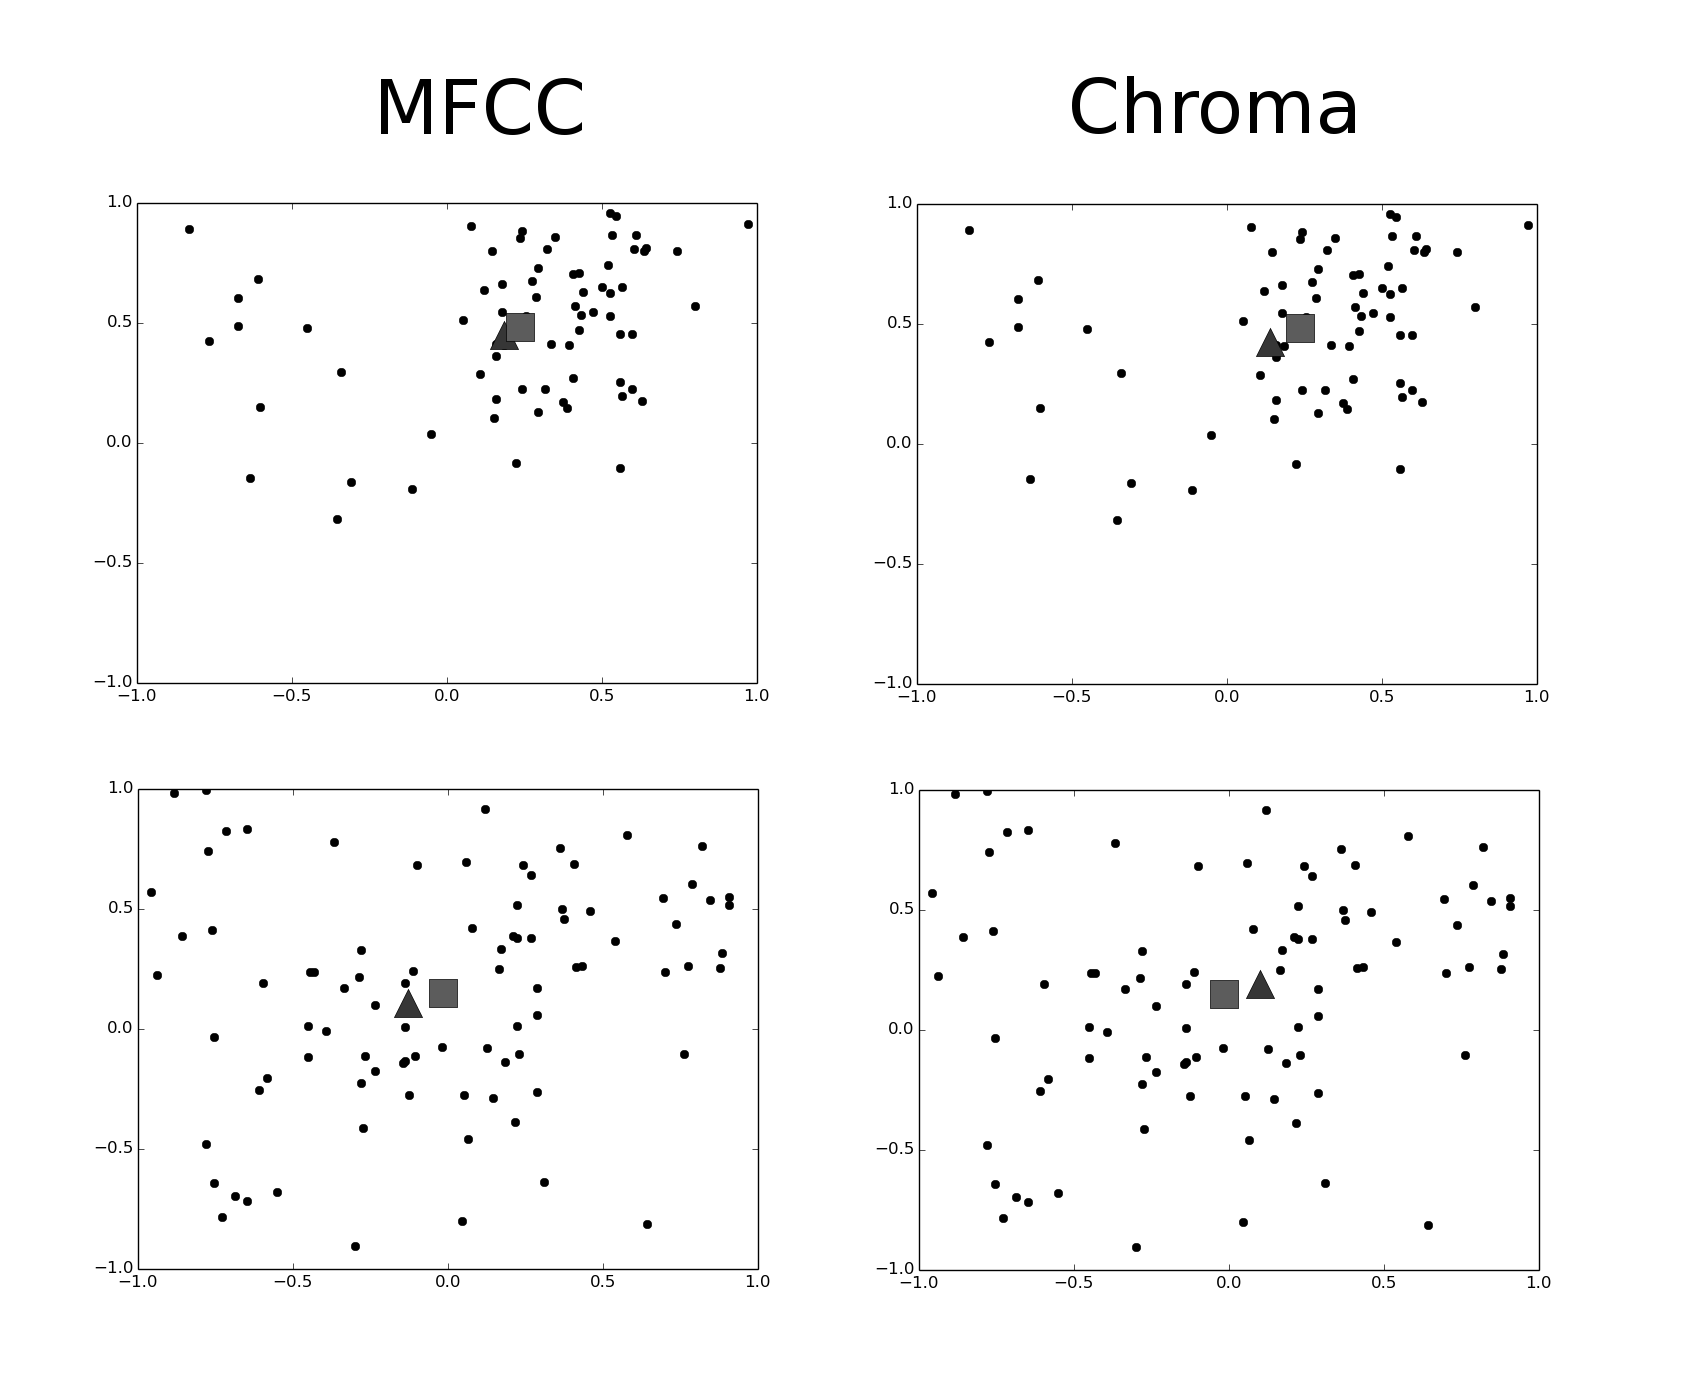
\includegraphics[width=80mm]{graphs1.png}
\caption{Image shows 4 valence-arousal spaces, where pleasantness raises from left to right on abscissa and activeness for bottom to top on ordinate axis. The first row shows prediction on songs with IDs 13 (first row) and 71 (second row) using MFCC and Chroma. The triangle presents regression algorithm prediction, where as the square marks mean value of all valence-arousal values gathered with survey. Dots indicate all gathered valence-arousal responses.}
\label{graphs}
\end{figure}

Results using regression algorithm are shown in table \ref{regressionresults}. For regression with MFCC and regression with Chroma average distance between estimated and mean valence-arousal value was calculated. We also provide the average distance to nearest value in dataset and the average distance between the mean valence-arousal point and the prediction, measured in the size of the standard deviation of data. Same algorithm was also used on the features Schmidt et al. provides for Mood Swing dataset \cite{schmidt2011modeling} to compare results. 

The results show a better correlation between MFCC and valence-arousal than this between Chro\-ma and valence arousal. The table also shows significantly better results obtained on our dataset, compared to the results on the Mood Swing dataset.  

[novo]
We also performed a regression algorithm on chroma features calculated with the Compositional hierarchical model described in \cite{pesek2013chord}, what gave us the best results on a regression algorithm. The average distance is 0.1862, the distance to nearest value is 0.0719 and the distance measured in standard deviation is 0.4459. 

\newcolumntype{L}[1]{>{\raggedright\arraybackslash}p{#1}}
\newcolumntype{C}[1]{>{\centering\arraybackslash}p{#1}}
\newcolumntype{R}[1]{>{\raggedleft\arraybackslash}p{#1}}

\begin{table}[h]
\caption{Average distances between the predictions and the mean valence-arousal value shown separately for the valence and arousal arousal component. Distance for arousal is significantly smaller.}
\begin{tabular}{|L{1.2cm}|C{1.6cm}|C{1.6cm}| C{1.8cm}|}
\hline
 & MFCC & Chroma & MP Chroma \\
\hline
Valence & 0.1734 & 0.1826 & 0.1494\\
Arousal & 0.0871 & 0.0940 & 0.0898\\
\hline
\end{tabular}
\label{seperateresults}
\end{table}

The table \ref{seperateresults} shows the accuracy in predictions separately for valence and arousal values measured in average distance between prediction and mean valence-arousal value from dataset. Results indicate a more accurate prediction of the regression method for arousal component.

\section{Conclusion and future work}

We gathered well annotated dataset with a lot of responses with online survey, which will be publicly available prese\-ntly. It contains participants' demographical data, users mood and color perception and most importantly, a significant amount of mood and color responses per audio clip in the dataset. Each of these responses contains induced emotions and perceived emotions with valence-arousal values. It also contains color perception for audio. Unlike several others datasets ours will also provides audio clips used in survey, due to the copyright of the original audio. 

This dataset opens new possibilities for research mood evaluation from audio. Mood evaluation is an important for music recommendation systems based on mood. Personal background data of the participants in our dataset provides new possibilities to research usage of such data for the music recommendation.

We will shortly begin with the second run of survey. This survey will be presented in English language and will contains an additional set of audio clips. With the second run we intend to raise the number of responses per clip and enlarge number of audio clips in dataset. We also plan on comparing the collected data for English-speaking versus Slovene-speaking participants. We will continue testing the mood evaluation algorithms on data\-set and intend to develop a new method which considers demographic and background data of the annotators.

We will further explore correlation between mood and colors. We intend to develop a music visualisation, based on the results of our study. The visualisation will be used in music recommendation interfaces, substituting the text and other data on the user's screen with a visual representation of the audio.


\bibliographystyle{plain}
\bibliography{erkbib}{}

\end{document}
